% !TEX root = ../thesis.tex
\chapter{Simulating Cyber-Physical Systems in the Virtual-World}
% Describe what better CPS tools would provide - environmental simulation, trained environment models, virtual environments, cross-environment simulation

Testing and understanding how the environment interacts with a sensor network and vice-versa relies on placing the devices in the target environment and waiting for or creating the desired phenomena to interact with the network. Phenomena can include events such as movement of devices/objects, passive or active interaction with people (pressing buttons, triggering motion sensors), or other sensor events. Human mobility also poses difficulties, including participant recruitment, health and safety requirements and limitations, physical limitations, etc. Hence, performing tests in the real-world is time-consuming, costly and often impractical. 



In this chapter we present a novel co-simulation approach to this problem, designed taking into consideration the the requirements discussed in chapter \ref{chap:framework}. The co-simulator is built upon a publish-subscribe event-bus, integrating a high-performance 3D game engine, Unreal Engine 4, with an existing sensor network simulation platform, Cooja, to create a dynamic, flexible and more reliable end-to-end simulation solution for testing cyber-physical systems in their target environments. Harnessing a 3D game engine, we introduce simulated cyber-physical systems into virtual reality, with realistic real-time physics, dynamic and controllable phenomena, AI agents, and realistic lighting effects. The co-simulation platform adopts the publish-subscribe architecture, supporting an open, flexible and expandable platform for co-simulation development.


% In this chapter we present and evaluate a novel approach to this problem, integrating a freely available high-performance 3D video game engine (Unreal Engine 4) with an existing sensor network simulation platform (Cooja), creating an end-to-end simulation solution for realistic testing of sensor networks in their target environments. By integrating a 3D game engine, we are introducing sensor network simulations into virtual reality with a real-time and dynamic virtual world, utilising the game engine's realistic physics, lighting and artificially intelligent people and crowds to influence and test the deployed sensor network.

% In the following section we describe in detail our novel 3D simulation platform, Ard\'{a}n, discussing the various features and tools it provides. Section 2 discusses the requirements which we believe to be vital for 3D simulation platform development. Section 3 describes the design and architecture of Ard\'{a}n, followed by an example case study for testing and deployment in section 4. We subsequently present a performance evaluation and discuss the challenges involved in developing the Ard\'{a}n platform, in sections 5 and 6 respectively.
\section{Problem} % (fold)
\label{sec:problem}
Cyber-physical systems are deployed in physical environments, interacting with the surrounding physical infrastructure to provide services for nearby inhabitants, such as heating, lighting, security, fire and environmental safety. Significant research within WSN and CPS simulation has focussed on accurately simulating and emulating hardware devices, the network and power consumption, with great success \cite{cooja, tossim}. Alternatively, test-beds offer testing with real devices and over a real radio network, sometimes with tunable network inference\cite{dependibilityTestbedChallenge} or other conditions, such as temperature\cite{TempLab}. However, these tools and techniques used to develop, test and analyse such systems don't simulate the physical environment, its inhabitants or their mobility. 

The rest of this section discusses the issues related to simulation and test-beds in more detail.

\subsection{Simulation Issues} % (fold)
\label{ssub:simulation_issues}

% subsubsection simulation_issues (end)
When testing in simulation, typically the environment data is fed into simulations using recorded sensor data (traces) from an existing deployment, field study\cite{bridge,Gaglione2018}, or is fabricated based on a developer's conceptual model and testing needs. However, using this approach is not without issues.

Acquisition of traces is a difficult and time consuming task, as traces need to be recorded from existing real-world deployments or field studies; the former may not match the target network, and the later can be time-consuming, expensive, dangerous, or inconvenient to perform thoroughly. Once these traces are recorded, they are static and dependent on the fixed position they were recorded from, unable to be modified after-the-fact, e.g., to adjust for moving a sensor in a simulation.

In the case of fabricating traces, these are highly dependent on the desired phenomena a developer is attempting to model and their understanding of it, hence, modelling complex phenomena such as gravity or thermal dynamics by hand is a non-trivial task. Instead developers may choose to imitate certain phenomena with less precision or accuracy, which may result in a disconnect between the test and its performance in the real-world.

Regardless of the method for creating traces, creating comprehensive traces which cover a large number of test scenarios across different scales and layouts of a network is extremely time-consuming and often not feasible, e.g., gathering real traces on a bridge with limited access \cite{Gaglione2018}. Hence, the total coverage of tests for these different variables are reduced.

\subsection{Deployment and Test-bed Issues} % (fold)
\label{ssub:deployment_and_test_bed_issues}

% subsubsection deployment_and_test_bed_issues (end)
For CPS involving human and device mobility, deployment and test-beds\cite{wisebed1,wisebed2,TempLab,dependibilityTestbedChallenge} are not only time-consuming and expensive to deploy, but also are limited by health and safety, people recruitment, location availability, and scalability issues.

Testing involving people needs to ensure strict health and safety guidelines and laws are adhered to, requiring participants to be safeguarded against possible injury and death, thus, testing situations in which poses a threat to participants can't be carried out, e.g., testing crowd based scenarios or scenarios involving hazards such as fire or flooding. Similarly, ethical guidelines must also be followed when involving people, requiring developers to consider guidelines such as VIP ethical guidelines used in human computer interaction (HCI) studies\cite{blandford2008_controlled_experiments,blandford_pretareporter}: Vulnerability, care must be taken when recruiting participants young, elderly, or people with particular conditions; Informed consent, participants must be aware of the experiment and be allowed to withdraw at any time; Privacy and confidentiality must be observed, with participants data anonymised.

It's not possible to run tests with real people in real evacuation scenarios, due to the health and safety risks mentioned above. Instead we can try to simulate these scenarios in the real-world using fire-drills, a significantly lower risk to participants; however, fire drills by nature have an impact on how people may act during an evacuation. Similarly, people may become familiar with the environment the more tests they perform, which could affect their reaction time and the choices they make. 

Recruiting participant also poses a challenge for larger test scenarios, in which recruiting, organising and managing large numbers of participants requires significant planning, approval and management.Similarly, running large numbers of tests with even a small number of people may simply not be possible due to time constraints, thus, only a core set of tests may be carried out instead, limiting the scope.

Exclusive access to target locations prior to full deployment for testing can be difficult at peak times, requiring out-of-hours testing on weekends or evenings. This can have a knock on impact for recruiting participants.


In the rest of this chapter, we introduce a novel CPS co-simulation platform that has been developed to tackle the issue of simulating a CPS with realistic, dynamic and flexible environment input, described above; the design of the co-simulation platform is based on the framework described in chapter \ref{chap:framework}.


% section problem (end)
\section{A Virtual Reality Co-Simulation Platform} % (fold)
\label{sec:a_3d_co_simulation_platform}

To meet the needs of simulating a CPS pre-deployment with realistic, dynamic and flexible environment input a novel approach is needed, capable of simulating both the cyber, a CPS, and the physical, the environment, humans and phenomena; hence, we designed and built a co-simulation platform, integrating a WSN simulator with a 3D game engine to close the cyber-physical loop in simulations. 

\subsection{The 3D Game Engine: Unreal Engine 4} % (fold)
\label{sub:a_3d_game_engine}

% subsection a_3d_game_engine (end)
Using the 3D game engine, we're able to create vivid and realistic models of the real world, involving complex physics, AI pedestrians and crowds, physical destruction, and lighting. In games, films and TV these effects are used purely for creating immersive experiences which can trick the viewer into suspending disbelief; within a simulation these can be instead used effectively to create living simulations grounded in reality. 

Using the game engine's physics engine, we're able to build 3-dimensional physical environments, from the size of a corridor up to a whole city, complete with realistic physical properties and effects, such as gravity, momentum, friction and collisions between objects in real-time. Leveraging the real-time physics we can create dynamic and reactive physical input for our cyber simulations. Using the physics engine we can also simulate destructible environments and buildings, dynamically reacting to virtual earthquakes, explosions or other destructive phenomena.

Like many game engines, the Unreal Engine also includes a suite of tools to support creating responsive AI characters, capable of dynamic and reactive behaviour in real-time. Utilising these tools we can simulate human-centric CPS such as in offices, schools or stadiums, with pedestrians and crowds exhibiting desired behaviours, such as goal-based movement, avoidance, herding, panic, etc.

Unreal Engine can also simulate realistic lighting effects, such as refraction, bloom, shadows, fire and smoke; lighting can have a significant impact within an environment, such as a room or building, providing participants with a clear view when natural or artificial light is available or poor visibility when fire and smoke fill a room. when performing human-centric simulations,  allowing viewers to understand how lighting and visibility may be affected by different sources of light (sun, lamps, lights, fire) and in different scenarios, day-to-day office, fire evacuation etc. 
Using these features, we can:


Using the input from the 3D game engine to drive the CPS simulation which can then drive change in the virtual world, creates truly dynamic and reactive closed-loop simulations; such a system removes the need for developers to gather, fabricate, modify or update individual sensor traces. This gives developers more time to focus on building better CPS based on their tests, than building the tests.

We believe utilising a 3D game engine to drive the CPS simulation can help resolve the simulation issues described previously, section \ref{ssub:simulation_issues}. Developers can model 3D environments which realistically match the design, layout, scale and conditions of their desired target environment, from single rooms to whole buildings. This enables developers to capture sensor traces from anywhere in the environment and virtually experiment with device placement at any time, without the difficulties associated with accessing real deployment environments.

Leveraging the 3D game engine's physics engine, it's possible to create dynamic, reactive and realistic sensor traces, relieving the burden on the developer to create ``realistic'' sensor traces. For example, calculating when a person walking at 2km/h will intercept motion sensors lining a CPS-enhanced lit corridor. Because of this testing out various scenarios is scalable as the number of devices or scenarios increases, as devices or AI are added, moved or removed, the simulation will dynamically adapt and create new traces for the relevant sensors.

Using the 3D game world it's possible to run tests not only at any time, no longer restricted by real-world access hours, but also possible to reduce testing time by simulating the virtual-world at faster than real-time.

%  \begin{description}
%   \item [Acquisition] - developers can model 3D environments which match the design, layout and conditions of their target environment.
%   \item [Dynamic and Reactive] - new traces are generated in real-time based on the CPS and environment as it changes, be it a new layout or pedestrian behaviour reacting to the CPS or other phenomena.
%   \item [Reliable] - the game engine simulates a virtual world grounded by realistic physics and lighting. Therefore, relieving the burden on the programmer of creating realistic input models, e.g., calculating when a person will intercept motion sensors as they walk down a corridor. AI people and crowds can be programmed based on desired needs e.g., herding, follow, avoid behaviours.
%   \item [Comprehensive] - simulations can be carried out faster than real-time, combined with the dynamic physics-based world enables many different scenarios to be tested out in significantly less time.
%   \item [Scalable] - as new devices are added or existing ones moved, the simulation dynamically adapts and creates a new trace.
% \end{description}

Similarly, we believe this co-simulation approach can begin to address the deployment and test-bed issues described in section \ref{ssub:deployment_and_test_bed_issues}.

Virtual tests involve virtual people, hence, health and safety rules need not apply. However, one envisions they could apply to some extent if real people are used for virtual reality (VR) tests, but with much less risk attached e.g., real people can't be physically burned by a virtual fire, although they may experience VR sickness.

Participant recruitment is a non-issue, within a 3D game engine world, 100's of AI participants can be created as and when needed, no bribing or ethics paperwork necessary. 

As discussed above location access is resolved by modelling it in 3D, based off a floor-plan, requiring no access to the real physical location. Alternatively, a one-time measurement survey can be carried out with minimal interference caused.

It is possible to run tests with large numbers of people 24/7, without issue or complaints, scheduling issues or location availability issues.

Whilst achieving 100\% realistic people and crowd behaviour may not be possible using a game engine's AI, we can use AI people and crowds to mimic previously observed behaviour accurately, enabling more consistent simulations when compared to real people in fake or ``drill'' scenarios, e.g., virtual people can be told to panic or mimic herding behaviour, whereas real people may not exhibit this behaviour in non-life-threatening scenarios. This enables developers to test for these different behaviours and scenarios which affect them. However, the AI behaviour may not reflect the true unique and complex reactions of a real person and crowd in real scenarios.

\subsection{The WSN/CPS Simulator: Cooja} % (fold)
\label{sub:a_wsn_cps_simulator}
Like previous physical simulator approaches \cite{6815220,simulink}, we could use a standard programming language and environment to program and model the WSN component, such as the language used within the game engine, C++. However, this approach has several drawbacks.

Programming in a non-WSN or CPS language and environment requires porting to the desired platform when transferring from testing to deployment. This can introduce translation bugs and vary in difficulty depending on the differences in language, environment and especially on the differences in programming paradigm or memory model e.g., event-based or imperative, static or dynamic memory. 

Similarly, many issues in WSN and CPS depend on the hardware and performance constraints of the deployment devices, which have severely limited CPU, RAM, ROM and battery power. Hence, simulated nodes without consideration or an accurate simulation of these constraints, i.e., running natively on a full desktop machine, won't provide an accurate representation of how the software will run once deployed on a set of constrained devices.

WSN/CPS rely on their radio network for communicating between nodes within a network, which also has a significant impact on other aspects of the device, such as performance, duty cycle and battery life.


Utilising the Cooja WSN simulator enables the co-simulation platform to build upon the tool to create a powerful testing platform which developers can test on before seamlessly deploying to real devices in their target environment.

Cooja nodes are programmed in the Contiki C language, hence, the same code can be deployed for simulated nodes as for deployed nodes. This enables a seamless transition between simulated and real nodes and removes the translation bugs and issues related to translating between a simulated language and a real node language.

Cooja nodes can be simulated at various accuracy levels, using the same code, dependent on the simulation level needed (hardware emulation, simulation or natively) and the available computing power of the host simulation PC. Dependent on a developers needs this can help test accurately using hardware emulation, or test scalably using less hardware-accurate simulation but with significantly larger network sizes, 10's vs 100's devices.

Cooja simulates the radio medium with several optional radio simulation models, enabling developers to test simple and complex radio scenarios, with varying RSSI and interference models to reflect real-world radio environments.

% subsection a_wsn_cps_simulator (end)
% section a_3d_co_simulation_platform (end)

\section{Co-Simulator Design}
\label{sec:Design}
Discussed in chapter \ref{chap:framework}, the co-simulation platform is designed in an open, component agnostic fashion, i.e., the platform encourages the interoperability of different simulation platforms, specifying clear abstractions and boundaries between components and uses a publish / subscribe bus to communicate. The goal is to create a plug-n-play platform that can support the use of different simulation, analytical and game engine tools, with our implementation providing an example construction.

\subsection{WSN Simulator Component} % (fold)
\label{sub:wsn_simulator_component}

The WSN simulator, Cooja, performs the hardware, software and radio network simulation for each node within a WSN in the co-simulation. 
Users select the hardware they wish to deploy there application code, software, to, which is then compiled for the desired platform. Depending on the level of accuracy, host PC performance and size of the desired network, developers can select the hardware simulation level they wish the node to be simulated at, which ultimately dictates whether the code is compiled to the target or host architecture. This enables developers to sacrifice hardware accuracy for a larger simulated network.

\subsubsection{Radio} % (fold)
\label{ssub:radio}

Radio simulation is performed entirely within Cooja, relying on the built-in radio models and distance between nodes to determine node RSSI and packet-loss. However, to enable dynamic and mobile nodes, Cooja subscribes to node location updates; when a nodes position is updated by other components, such as by being moved in the virtual world, the radio model is updated any any subsequent radio activity is affected by this.

To provide other components with information about the radio environment, including transmissions and successful or interfered receives, the radio component publishes all radio state to the radio topic. 

Utilising the game engine's knowledge of the 3D world and obstructions between nodes could improve the fidelity of the radio simulation, however, this remains as future work. Kokkinis et al.\cite{trunetWireless} have demonstrated the use of 3D models of target environments to simulate an accurate radio model based on obstructions and their material types. Once the 3D model is built within the game engine component, the model can be exported to the TruNet tool to calculate the radio model and then import back into Cooja providing an accurate radio model based on the virtual environment.


% subsubsection radio (end)
\subsubsection{Location and Movement} % (fold)
\label{ssub:location}

Each node is configured with an initial 3D location, used in the radio simulation to calculate radio interference. The location is exposed to other co-simulation components via pub/sub topics which Cooja is subscribed to. This enables it to be updated at any time by other co-simulation components, in this case the game engine. This provides developers the ability to test scenarios with dynamic mobile nodes, which affect the radio simulation within Cooja.

It is also possible for nodes with inertial measurement units (IMU) to receive updates, to inform applications of any 3D movement, discussed further in the following section.
% subsubsection location (end)

\subsubsection{Hardware Interfaces - Sensors and Actuators} % (fold)
\label{ssub:hardware_interfaces_sensors}

Hardware interfaces which normally interact with the physical world, such as motion, acceleration, light sensors and buttons, are exposed as virtual hardware interfaces to other co-simulation components via pub/sub topics.

\missingfigure[figheight=7cm]{Will show how - Node hardware interfaces connect to other components via a publish/subscribe bus.}
\begin{figure}[ht]
  \centering
  \includegraphics[width=\textwidth]{img/Eventbus.pdf}
  \caption{Node Event bus}
  \label{fig:compression}
\end{figure}
Data related to input interfaces can be published to by co-simulation components, to which Cooja subscribes and distributes to the relevant nodes, such that when a node queries an on-board sensor, the most up-to-date reading is available, from within the component. This also ensures response time for hardware interface requests is kept to the absolute minimal, requiring no cross-component calls (i.e., network calls) to retrieve data. However, this method could result in applications reading delayed, stale data, by approximately the RTT/2 between publisher and subscriber; in applications where sensor data is high frequency and ephemeral, this approach induce a time-delay effect when comparing simulated vs real-world tests. This delay will be explored in the evaluation, section \ref{sec:architecture_evaluation}. 

Similarly, data related to output interfaces, such as LEDs or actuators, is published by Cooja to the relevant per-interface topics; allowing subscribed components to be updated in real-time of such hardware events, which can then be: actioned in a virtual world component, such as turning on a light, opening a door or activating an alarm; or recorded by a logging or analytical component for further analysis.


% subsubsection hardware_interfaces_sensors (end)
% subsection wsn_simulator_component (end)

\subsection{3D Game Engine Component} % (fold)
\label{sub:3d_game_engine_component}
The 3D game engine component, Unreal Engine 4, is responsible for simulating the 3D virtual world and the physics, lighting and people within it. It also models the physical manifestation of the nodes and their exposed hardware interfaces i.e., sensors and actuators.

\subsubsection{Virtual Node Model} % (fold)
\label{ssub:virtual_node_hardware}
Within the virtual world we can choose to model node hardware to an accurate scale, or not. This allows for developers to choose physical accuracy when required for scenarios which may involve mobile nodes that can be affected by physics and collisions with the environment. On the other hand, we can sacrifice realism by increasing a nodes scale; this can help the visual locatability of a node and visibility of any information on the device, such as LEDs or an ID.

Figure \ref{fig:sensor_scales} shows three different scales of the basic sensor node model we designed. The model is designed as a simple cuboid with large LED lights on the top of the device, matching those typically found on a sensor node (TelosB Mote).
\begin{figure}[tbh]
   \centering
   \includegraphics[width=\textwidth]{img/sensorScales.png}
   \caption{Variable sensor scales, providing either physically accurate sized devices or more visible devices}
   \label{fig:sensor_scales}
 \end{figure} 

Within the virtual world, nodes can be set to either: static, its location is fixed and is not affected by physics; moveable, it can be acted upon by the physics engine e.g., fall due to gravity, react from a collision; or attached to another entity, such as a person or vehicle, moving as they move. This enables nodes to be dynamic mobile nodes reacting to the virtual environment.

% subsubsection virtual_node_hardware (end)

\subsubsection{Virtual Node Hardware Interface} % (fold)
\label{ssub:virtual_hardware_interface}
A node's representation within the game engine can sense and actuate within the virtual world via their virtual hardware interfaces. A node can be assigned multiple interfaces, each of which can publish or subscribe to updates on the relevant pub/sub topics with their associated node's ID. 

In the virtual world these hardware interfaces can programmatically sense the virtual world using primitives available within the game engine, shown in figure \ref{fig:collisionTypes}, such as trigger boxes, detects when entities pass in and out of an invisible non-colliding 3D shape; collisions, triggers an event when an entity collides with something in the environment; and ray casts, casts a line from a point in space, typically perpendicular to the face of an object, detecting any objects which it intersects with along the line's path. 

Figure \ref{fig:collisionTypes} demonstrates these different types of primitives available to developers to simulate physical sensors. Starting from the left, an agent is seen walking down a corridor and passes into a cuboid shaped trigger box, which upon happening, triggers an event, much like a motion sensor. Within the game engine the trigger box can be any shape, is invisible, allows objects to pass through them and each event provides any objects associated with causing the trigger - figure \ref{fig:motionSensor} shows a conical shaped trigger box simulating the field-of-view of a typical motion sensor. Using a trigger box, one could simulate a simple motion sensor, detecting when objects pass through its field of view, or enhance it by enabling it to recognise the names or types of objects or people which pass through it. Moving to the right, a ball is falling and colliding with another cube, this time triggering an event as it collides and ricochets off, upon colliding it's possible to detect the force of impact and any objects associated with the impact, providing the ability to simulate a sudden motion or vibration sensor (piezo sensor). Lastly, on the right is a ray-cast, starting from an object and passing through the sphere and person. Ray-casts have a configurable distance, stopping at either the nth object or at a set distance, returning all objects it intersects, from which a distance can be calculated.

\begin{figure}[tbh]
  \centering
  \includegraphics[width=\textwidth]{img/collisionTypes.pdf}
  \caption{A visual example of three different types of physics detection primitives available in a game engine: trigger boxes, collisions and ray-casts.}
  \label{fig:collisionTypes}
\end{figure}

Using these game engine primitives, developers can model a variety of sensors to desired varying degrees of accuracy e.g., a PIR sensor could use a trigger box to detect when a person enters its range, a distance sensor could use a ray-cast to detect distance to the first object it intersects, or a vibration sensor could use collisions to detect vibrations forces when it is hit. These and other primitives give developers the power to experiment with different sensor types, accuracies and capabilities, which may not be available to them or exist. Sensors are assigned to a virtual node's sensing port, associating a sensor with a unique node ID.

For performing actuation, a virtual actuation object, such as a light, alarm or door, is assigned to a node's actuation port. By default a node exposes 3 standard actuation ports, one for each LED built into a typical node. To perform actuation, another component simply publishes to the relevant actuator topic, which the targeted node then receives and performs the actuation in the virtual world.

\begin{figure}[tbh]
  \centering
  \includegraphics[width=\textwidth]{img/motionSensor.png}
  \caption{Motion sensors with their field-of-view visible.}
  \label{fig:motionSensor}
\end{figure}

Within the co-simulation platform we consider the following initial sensor and actuator types:
\begin{description}[topsep=0pt]
  \item [Button] - A physical button sensor can be directly interacted with by people, both AI and controlled, when in range. When pressed an event is triggered in the game engine.
    \begin{description}[topsep=0pt]
      \item[Type:] Triggered by an event. 
    \end{description}
  \item [Distance] - A distance sensor uses a single ray-cast to measure the straight-line distance from a point until the first object it hits. The distance sensor runs at a specified frequency, e.g., 20Hz.
  \item [Trip] - A trip sensor uses trigger box, several pixels wide and the length of the space, which upon an object crossing into it triggers an event within the game engine.
  \item [Motion] - Similar to a trip sensor, a motion sensor uses a trigger box in the shape of the motion sensor field-of-view, e.g., conical. When a human passes into, through, or out of it, it triggers an event. The range and sensitivity of the trigger box can be adjusted by developers. Also the class of detection can be changed from human to all objects, depending on the type of motion sensor being mimicked, PIR or ultrasonic respectively.
  \item [Presence] - A presence sensor can be thought of as an ultra sensitive human motion detector (detecting even still people) which can also detect the identity of the detected people. Similar to the motion sensor, human entities can be detected and also identified by programmatically reading the identity of any people within the range of the sensor. 
  \item [IMU] - Each node within the game engine knows its own 3D location, rotation and acceleration information, updated at each game tick. Using this information a node can simulate an inertial measurement unit sensor.
  \item [Temperature] - Unlike other sensors, the temperature sensor has no native primitive within the virtual world, as video games rarely model temperature. As a primitive, temperature could be modelled within a building by dividing the area into cuboids, matching the size of a room. As the temperature increases within a room, a connected space's temperature will also be influenced, at a speed dependent on the size of the temperature differential.
  \item [Light] - A light actuator is connected to a light source in the virtual world, this could be a room light, spot light or lamp. The light source can be either a binary light or dimmable.
  \item [Sound] - An sound actuator is connected to a sound source in the virtual world, such as an alarm or beep. When triggered the sound is played continuously until turned off. 
 \end{description} 

Independent of the sensor type, either polling or event-based, data is published to the relevant sensor topic with the associated unique node ID, enabling other components to subscribe to these sensor updates. Whilst the event-based sensors only transmit sensor data upon being triggered by an event, such as a collision, or interaction, the polling sensors send sensor data updates at a fixed rate.
% subsubsection virtual_hardware_interface (end)

\subsubsection{Virtual Environment \& Physics} % (fold)
\label{ssub:virtual_environment}
Within the 3D game engine developers can build virtual replicas of their target environments using the built in modelling tools, or import 3D models previously built, or from other CAD software, such as Blender\cite{Blender} and 3DS Max. This allows developers to leverage existing designs and models, or create new ones from scratch and share them with others e.g., an office block benchmark.

Within these built environments, the game engine is responsible for controlling a nodes location, utilising the physics engine to dictate how and where a node moves within an environment, e.g., falling due to gravity, reacting to collisions with solid objects such as walls and people, etc.
% subsubsection virtual_environment (end)

\subsubsection{AI People and Crowds} % (fold)
\label{ssub:ai_people_and_crowds}
Using the game engine's built in tools, developers are able to create and place virtual people into the environment. When creating people developers can specify their appearance and other physiological attributes, including their physical model, height, weight, walking and running speeds. Each of these attributes can have a significant effect, as they would in the real-world, on how the virtual person moves and interacts with the environment, e.g., reducing a person's size can enable them to fit through smaller spaces, or increasing their weight and speed will increase the force impacted on other objects upon collision.


% subsubsection ai_people_and_crowds (end)


% subsection 3d_game_engine_component (end)
\section{Phenomena-on-demand} % (fold)
\label{sec:phenomena_on_demand}
Unlike existing approaches which utilise purely trace-fed and scripted approaches which are static and difficult to modify, this simulator enables dynamic phenomena generation based on the user input or scripted behaviour. 
By taking direct control of devices or people within the environment, developers can interact with and modify the simulation directly and observe how the dynamic simulation responds. This differs to trace-fed alternatives which require developers to manually change the input to sensors based on how they believe the environment has changed. 

For example, two sensors are placed within a school corridor to detect the pace of people walking past; the sensors communicate and calculate the walker's pace, displaying a red light to people running. In a trace-fed scenario, developers script sensor detection inputs to the two nodes. Developers may generate a test case for different speed walkers or multiple walkers. For each test case, the developers need to manually calculate and modify each trace-feed for each sensor individually. For our approach, developers need only change the speed of a person walking and observe the effects on the system. This approach provides a much more intuitive and scalable solution to testing with large numbers of devices and as the number of input sensors increase, in which trace-fed solutions become unmaintainable.  
% section phenomena_on_demand (end)

\section{Mobility} % (fold)
\label{sec:mobility}
Compared to traditional simulators, such as Tossim\cite{tossim}, Cooja\cite{cooja} and NS2\cite{NS2}, which facilitate mobility only through manual scripting, our co-simulation approach, leverages the 3D game engine to fully realise dynamic and realistic human and device mobility within virtual environments.

Within the game engine it is possible to create both static and mobile devices, allowing developers to specify whether or not external forces can impact upon a nodes position, such as gravity or collisions from other objects. If static, devices stay fixed in place at the point they were deployed, it's possible to adjust this position before running simulations, but once running the devices will remain stationary; this can be useful when mobile nodes aren't needed and ensures unexpected movement won't cause any issues.

When setting a device as mobile, the device act as if it would in the real world. The device has a weight attribute which affects how it reacts to collisions with other objects. As the device moves it will collide with other solid objects, such as walls, people and other devices. Devices can also be attached to other mobile objects, such as people or robots, creating truly mobile nodes, that can be used to mimic mobile devices in the real-world.

As described in the previous section, developers can create and place virtual people within their environments of all different sizes, shapes, weights, speeds, etc. For integrating human mobility into a simulation, developers can utilise the AI toolkit provided by the Unreal Engine. Human mobility can be programmed in C++ or the visual programming tool, blueprints, to design simple movement patterns, or complex and reactive AI behaviours. 

For example, to create a mobility behaviour that instructs agents to move between a set of locations at random, we first create and place several target locations within our environment. Next, we write, in either C++ or blueprints, a function to choose a random target location and then issue a move-to command to that location. Upon receiving this command, the agent will utilise the Unreal Engine's built-in navigation mesh to dynamically calculate the shortest route to that location.

\missingfigure[figheight=7cm]{Will show an example blueprint demoing how to create a simple move-to behaviour.}
For our indoor example we created several basic behaviours, including:

\begin{description}
  \item[Move to location] One or all people move to a specified location by the shortest route.
  \item[Roam] All people roam between rooms and the corridor, simulating basic movement within an office.
  \item[Evacuate] All people attempt to leave the building via the closest exit.
  \item[Avoid] People will attempt to avoid an individual or object, changing their path or moving out of the way as it approaches.
  \item[Follow/Herd] People will ignore their previous behaviour and follow an individual.
\end{description}
% section mobility (end)

\section{Communication} % (fold)
\label{sec:communication}
For communicating data between co-simulation tools we use an asynchronous event-driven approach, as previously outlined in the requirements chapter \ref{chap:framework}. Our event driven approach is actually realised using event-notification, event-based-state-transfer and event-sourcing techniques\cite{eventSourcing,eventDriven} to create an asynchronous responsive and flexible co-simulation platform. Using Apache Kafka\cite{apacheKafka}, a real-time stream-processing pub/sub system, each co-simulation tool publishes or subscribes to a set of topics, such as sensors, for updating sensor information; actuators, for updating actuation information; or people, for updating the locations of people.

Each topic will typically have only one publisher, a co-simulation component which is responsible for managing and updating information related to that topic; for example, the game engine is responsible for managing and updating device hardware information, such as location in the virtual world, and any sensor information, such as whether the motion sensor has been activated or is a button pressed. On the other hand, a topic may have many subscribers (zero, one or more), which rely on events published to that topic, for example, the Cooja simulator subscribes to the sensor topic for updates about a device's location which it then reflects in its network map to generate a new radio model.

To reduce inter-component coupling and reduce latency, we use an event-notification approach, requiring all components which control or manage an aspect of the co-simulation platform to publish to a known topic when any state related to it is updated by that component; topics and their related events can be seen in table \ref{tab:topics_table}. Using this approach we can avoid components from requiring knowledge about where their events of interest are coming from, enabling us to later swap out or add additional tools with minimal configuration changes. Similarly, this halves the round-trip-time (RTT) as a component does not need to issue a request for the event, i.e., remote procedure call (RPC) or request response, it is instead notified of the event as soon as it occurs.

To further reduce coupling and reliance on other components data-stores, we also take an event-based-state-transfer approach, requiring publishers to publish not only that the event occurred, but also an up-to-date snapshot of the state that changed. Upon receiving an event the component has all the event related data, thus, removes the need for subscribers to request any state information from the publishing component and it's data-store, further reducing any latency caused by an additional RPC call. However, this approach has the drawback of increased memory usage, requiring subscribers to keep up-to-date their own copy of any state received that is of interest.

Lastly, we implement event-sourcing, in which all changes to the state of the simulation are are published as events and recorded by the event stream, such that they can be used to roll-back or replay a simulation. Kafka durably persists events, writing them to a log on-disk, with a parameterisable sliding window retention period over the stream of events, before dropping old events to make space for new ones. On top of this, each component has a unique event stream token, pointing to the last event they have observed, which makes it possible for individual components to traverse the event stream as they wish; as new components are added to the stream at run-time, they can choose to process all events in the stream from the beginning, or simply start from the latest event. This creates a future-compatible platform, enabling developers to plug-and-play different components at run-time, test different configurations and observe behaviour using a variety of tools without the need to re-run simulations.

Using event-sourcing also opens up the possibility to replay isolated parts of a simulation; for example, we could replay the sensor topic, using it to drive a new simulation using the recorded inputs.

\begin{table}[hb!]
\begin{tabular}{c|c|c|c|c|c}
Kafka Topic & Event & Data & Type & Publisher & Notes\\\hhline{=|=|=|=|=|=}
\rowcolor{red!50} Sensor & Location & $x, y, z$ & double & Unreal Engine & \\\hline
\rowcolor{red!50} Sensor & Button & Pressed & bool & Unreal Engine & \\\hline
\rowcolor{red!50} Sensor & PIR & Activated & bool & Unreal Engine & \\\hline
\rowcolor{green!50} Actuator & LED & Brightness & uint & Cooja & \\\hline
\rowcolor{green!50} Actuator & Beeper & On/Off & bool & Cooja & \\\hline
\rowcolor{blue!50}Radio & Transmission & Source & addr & Cooja & \\
\rowcolor{blue!50}      &              & Destinations & addr[] &  & \\
\rowcolor{blue!50}      &              & Interfered Destinations & addr[] &  & \\
\rowcolor{blue!50}      &              & Packet & byte[] &  & \\\hline
\rowcolor{orange!50}Agent & Location & $x, y, z$ & double & Unreal Engine &\\\hline
\rowcolor{orange!50}Agent & Activity & Standing, Walking, Running & enum & Unreal Engine &\\\hline
\end{tabular}
  \caption{Topics available to publish and subscribe to using Kafka.}
  \label{tab:topics_table}
\end{table}

\subsection{Schema} % (fold)
\label{ssub:schema}
For the two components, the Unreal Engine 4 game engine and the Cooja WSN simulator, we have implemented plugins which publish and subscribe to the topics listed in table \ref{tab:topics_table}. Topics are based on sensor inputs, which drive the Cooja simulator; actuator commands, which drive the actuator devices in the Unreal Engine; and agent information, which provide contextual information regarding the behaviour of agents within the Unreal Engine.

Kafka is a schema-agnostic by design, simply carrying bytes from publishers to subscribers via topics, a durably persistent stream of events. Because of this we can group similar events together, benefiting from Kafka's total ordering guarantees, ensuring that when replayed, events within a topic will be ordered as received by the stream. 

Hence, it's necessary to create a defined but flexible schema for different components to communicate and ensure data is received in a correct and valid format. Because the events may contain different fields and types, the schema must be flexible, allowing fields to be omitted when not needed, removing the overhead of sending dummy or zero data. One option is to create a flexible schema using a text-based key-value schema such as JSON providing a human-readable and dynamic schema, however, for small and frequent payloads a text-based approach is hugely inefficient, requiring a text-based key for even the smallest payloads. JSON also requires runtime exception handling code to ensure the flexible and dynamically-typed schema doesn't crash the receiver, due to omitting, changing the types of or adding new fields. 



\begin{figure}[htb]
  \begin{verbatim}
enum MsgType : byte { LED = 1, LOCATION, RADIO, PIR, PAUSE, RESUME, SPEED_NORM, 
SPEED_SLOW, SPEED_FAST, RADIO_DUTY, FIRE, TEMP, SMOKE }

struct Vec3 {
  x:float;
  y:float;
  z:float;
}

struct RadioDuty {
  radioOnRatio:double;
  radioTxRatio:double;
  radioRxRatio:double;
  radioInterferedRatio:double;
}

table Message {
  id:int;
  type:int;
  location:Vec3;
  node:[RadioDuty];
  rcvd:[int];
  led:[int];
}
  \end{verbatim}
\end{figure}

Instead, the co-simulator uses a more efficient, forwards- and backwards-compatible binary serialising and de-serialising approach, Google Flatbuffers\cite{flatbuffers}. Flatbuffers serialises data efficiently by removing structural information from the buffer, requiring minimal overhead for schema information, as sending and receiving parties are required to agree on a schema ahead of time. Flatbuffers fields are strongly typed, so errors are handled at compile-time rather than requiring additional code for run-time checks. Unlike other binary serialisation protocols, such as Google Protobuffers\cite{protobuffers}, Thrift\cite{apachethrift} or Cap`n`proto\cite{capnproto}, which require an unpacking step on the receiving side before accessing the data i.e., one-copy read, flatbuffers requires no unpacking, resulting in zero-copy reads and faster processing of received buffers, ideal for real-time systems.
% subsection schema (end)
% section communication (end)
\section{Synchronisation} % (fold)
\label{sec:synchronisation}
Due to simulation speed-ups or slow-downs, due to performance or scheduling issues, simulations can run ahead or behind their expected run-time, i.e., at 1x real-time speed, a simulation might experience brief performance slow-downs and only simulate 9.5 seconds in simulation time within a 10 seconds of real-time simulation, leaving a lag of 0.5 seconds. To keep the simulations synchronised between components, components inform each other of one another's simulated time via the time topic. Upon receiving a time event from another component, if its simulated time is out with its own by a set threshold, then it can pause to allow for the other component to catch up.
% section synchronisation (end)



\section{Forward Time Control} % (fold)
\label{sec:time_control}
Using the Cooja simulator it's possible to run a simulation at a slower or faster than real-time rate, providing developers with more time to observe simulation or a faster completion time, respectively. Similarly, it's also possible to run a co-simulation in the same fashion, providing simulation speeds of 0.1x, 1x, 2x and 3x; which slows down or speeds up both the CPS simulation and virtual world simulation, enabling developers to run dynamic simulations with realistic physics in significantly less time than could be accomplished in the real-world. 

In simulation pausing is also possible, giving developers the power to stop the world, observe, and analyse what activity is occurring in the system and world. Unlike a paused video recording, within the game engine, developers are able to explore the 3D environment whilst the world is frozen, providing developers with the ability to be omnipresent within the simulation. In cases where a cause-and-effect may not be obvious from one viewing angle, a developer can pause and investigate the world to assess the true cause of some phenomena from multiple angles; for example figure \ref{fig:views} shows the same moment from three angles, over the shoulder, birds eye and a security camera style view.

When a speed change is issued within the game engine by the user, the game engine publishes the change of speed to the time topic, alerting other components. 

\section{Case Study}
\label{sec:Case Study: Corridor}

The purpose of the following case study is to demonstrate what development of a non-trivial CPS application is like using Ard\'{a}n, and how it enables developers to test and visualise different scenarios, by simply adding or moving devices or people in the simulation.

The case study focuses on controlling the lighting within a modern day office corridor, with the goal of striking a balance between energy efficiency, effective lighting and user comfort. The ideal corridor lighting scheme should provide a pleasant lighting scheme for users of the corridor, able to adjust based on ambient light levels, gradually illuminating as they progress through it, whilst also ensuring energy is minimised by turning off or reducing the brightness of unused or infrequently used parts of the corridor.

Thus, this provides an interesting and non-trivial task, due to the many ways in which the corridor can be entered/exited or moved around within in; people can enter from the beginning, end or from a room; people can move down the length of the corridor or directly from room to room; people often also stop in the corridor, spending time talking or waiting. Similarly, understanding the ideal number and placement for devices and sensors, and how it affects applications, such as power, reliability, robustness etc. Hence, providing effective lighting schemes can prove difficult to analyse and reason without rigorous testing.

The rest of this section will demonstrate and discuss the use of Ard\'{a}n to design, analyse and test for our target environment, the corridor, highlighting the features and benefits that the tool provides.


\begin{figure*}[t]
  \centering
  \subfloat[Over-the-shoulder view]{
    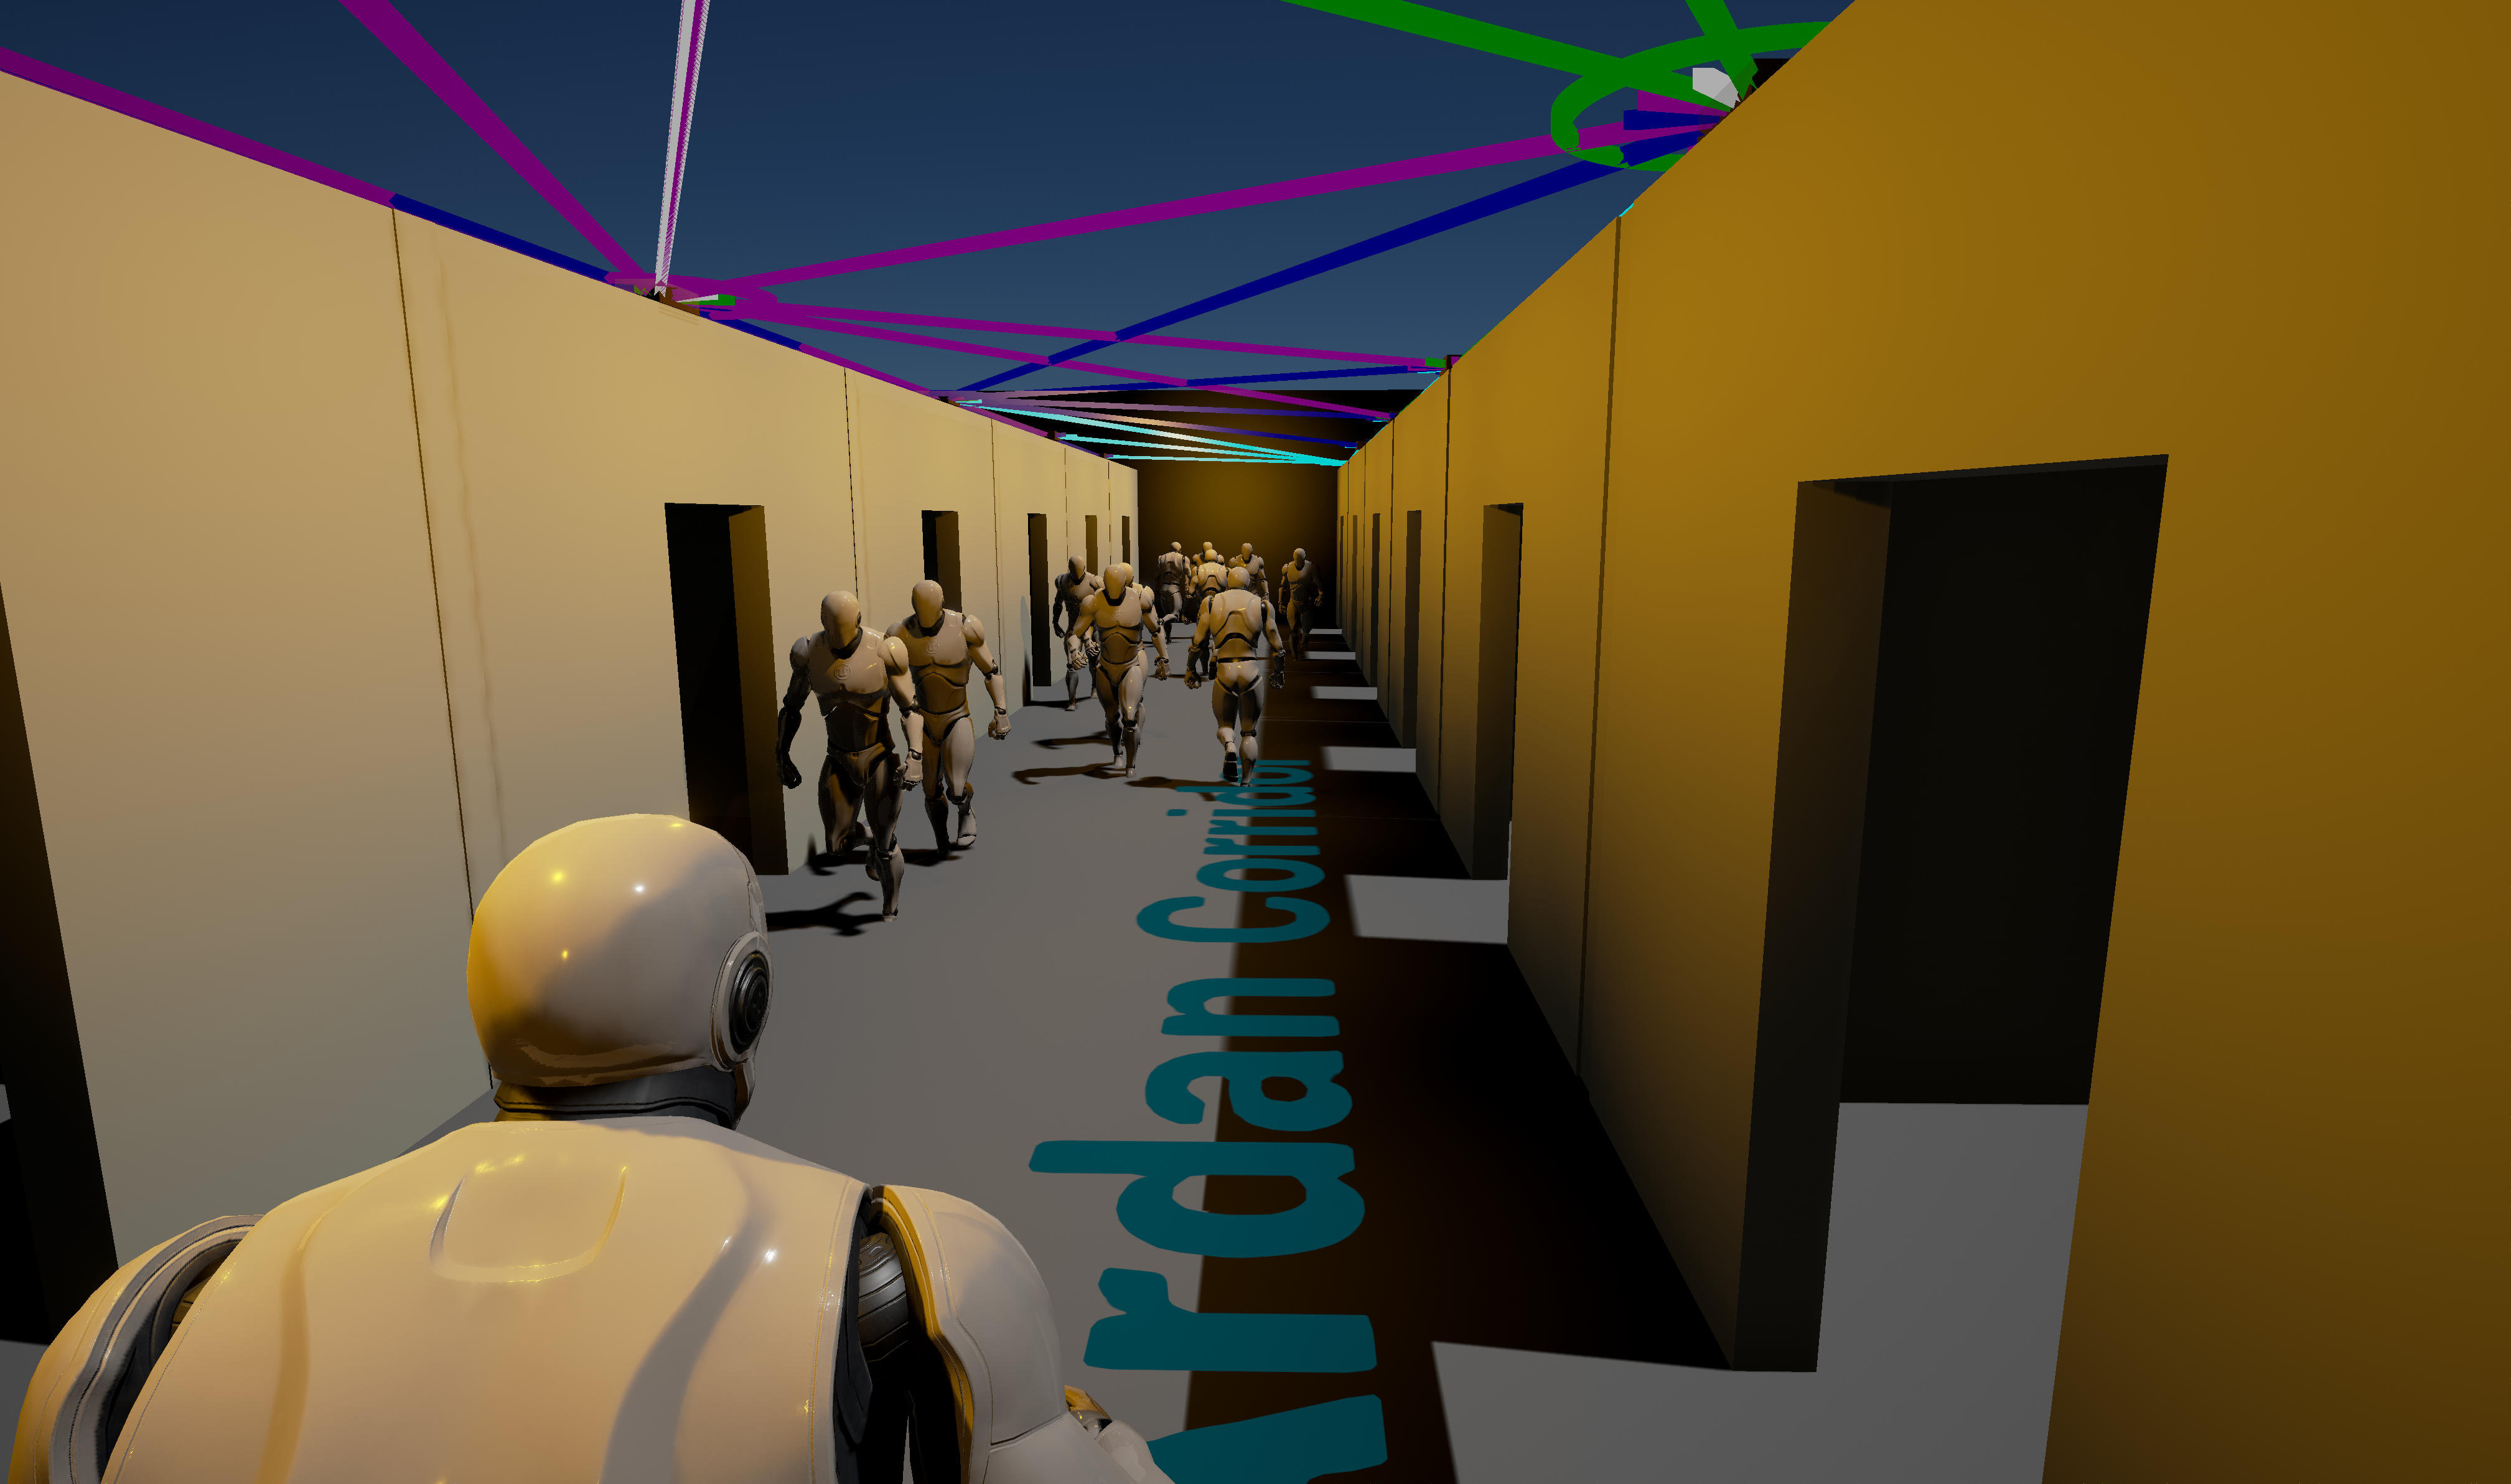
\includegraphics[height=2.6cm]{imgs/OverShoulder.jpg}
    \label{fig:birds_view}
  }
  \subfloat[Birds-eye view]{
    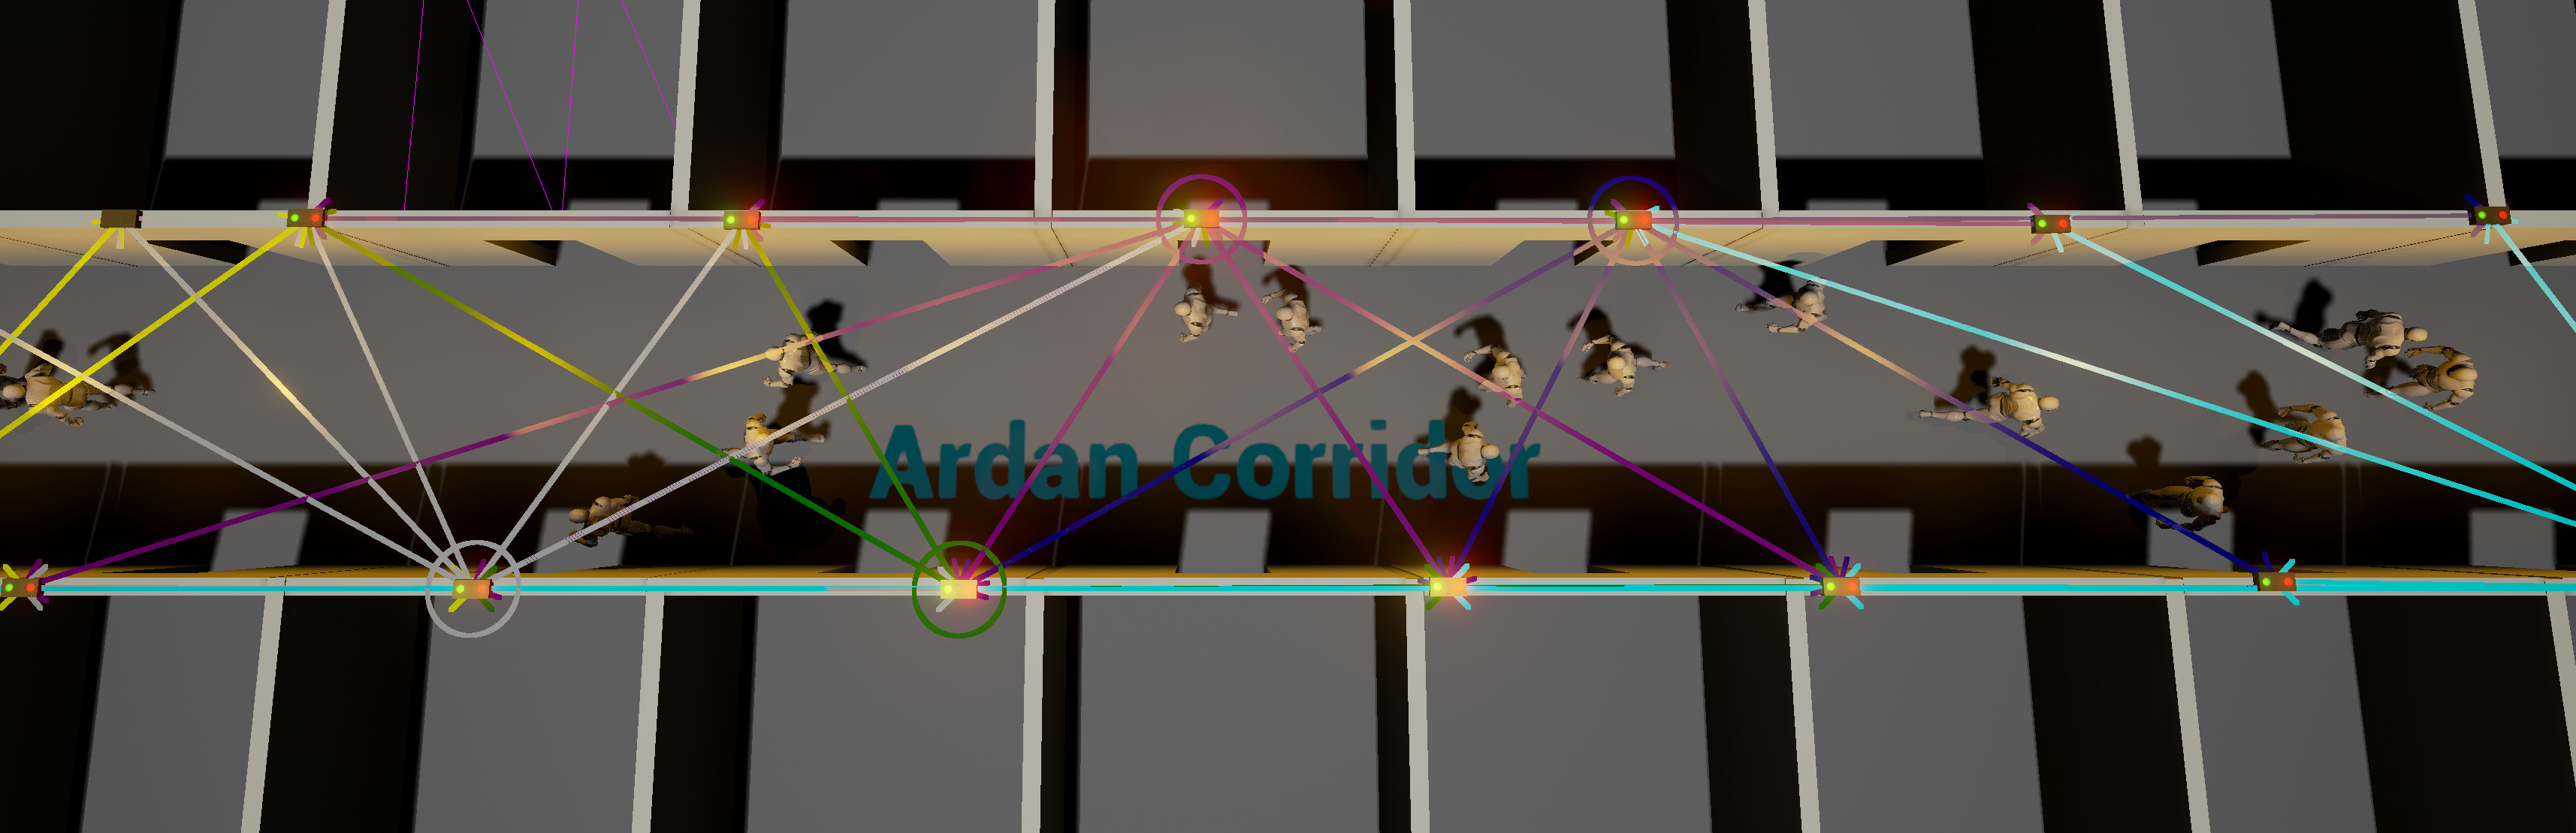
\includegraphics[height=2.6cm]{imgs/BirdsEye2.jpg}
    \label{fig:shoulder_view}
  }
  \subfloat[Camera view]{
    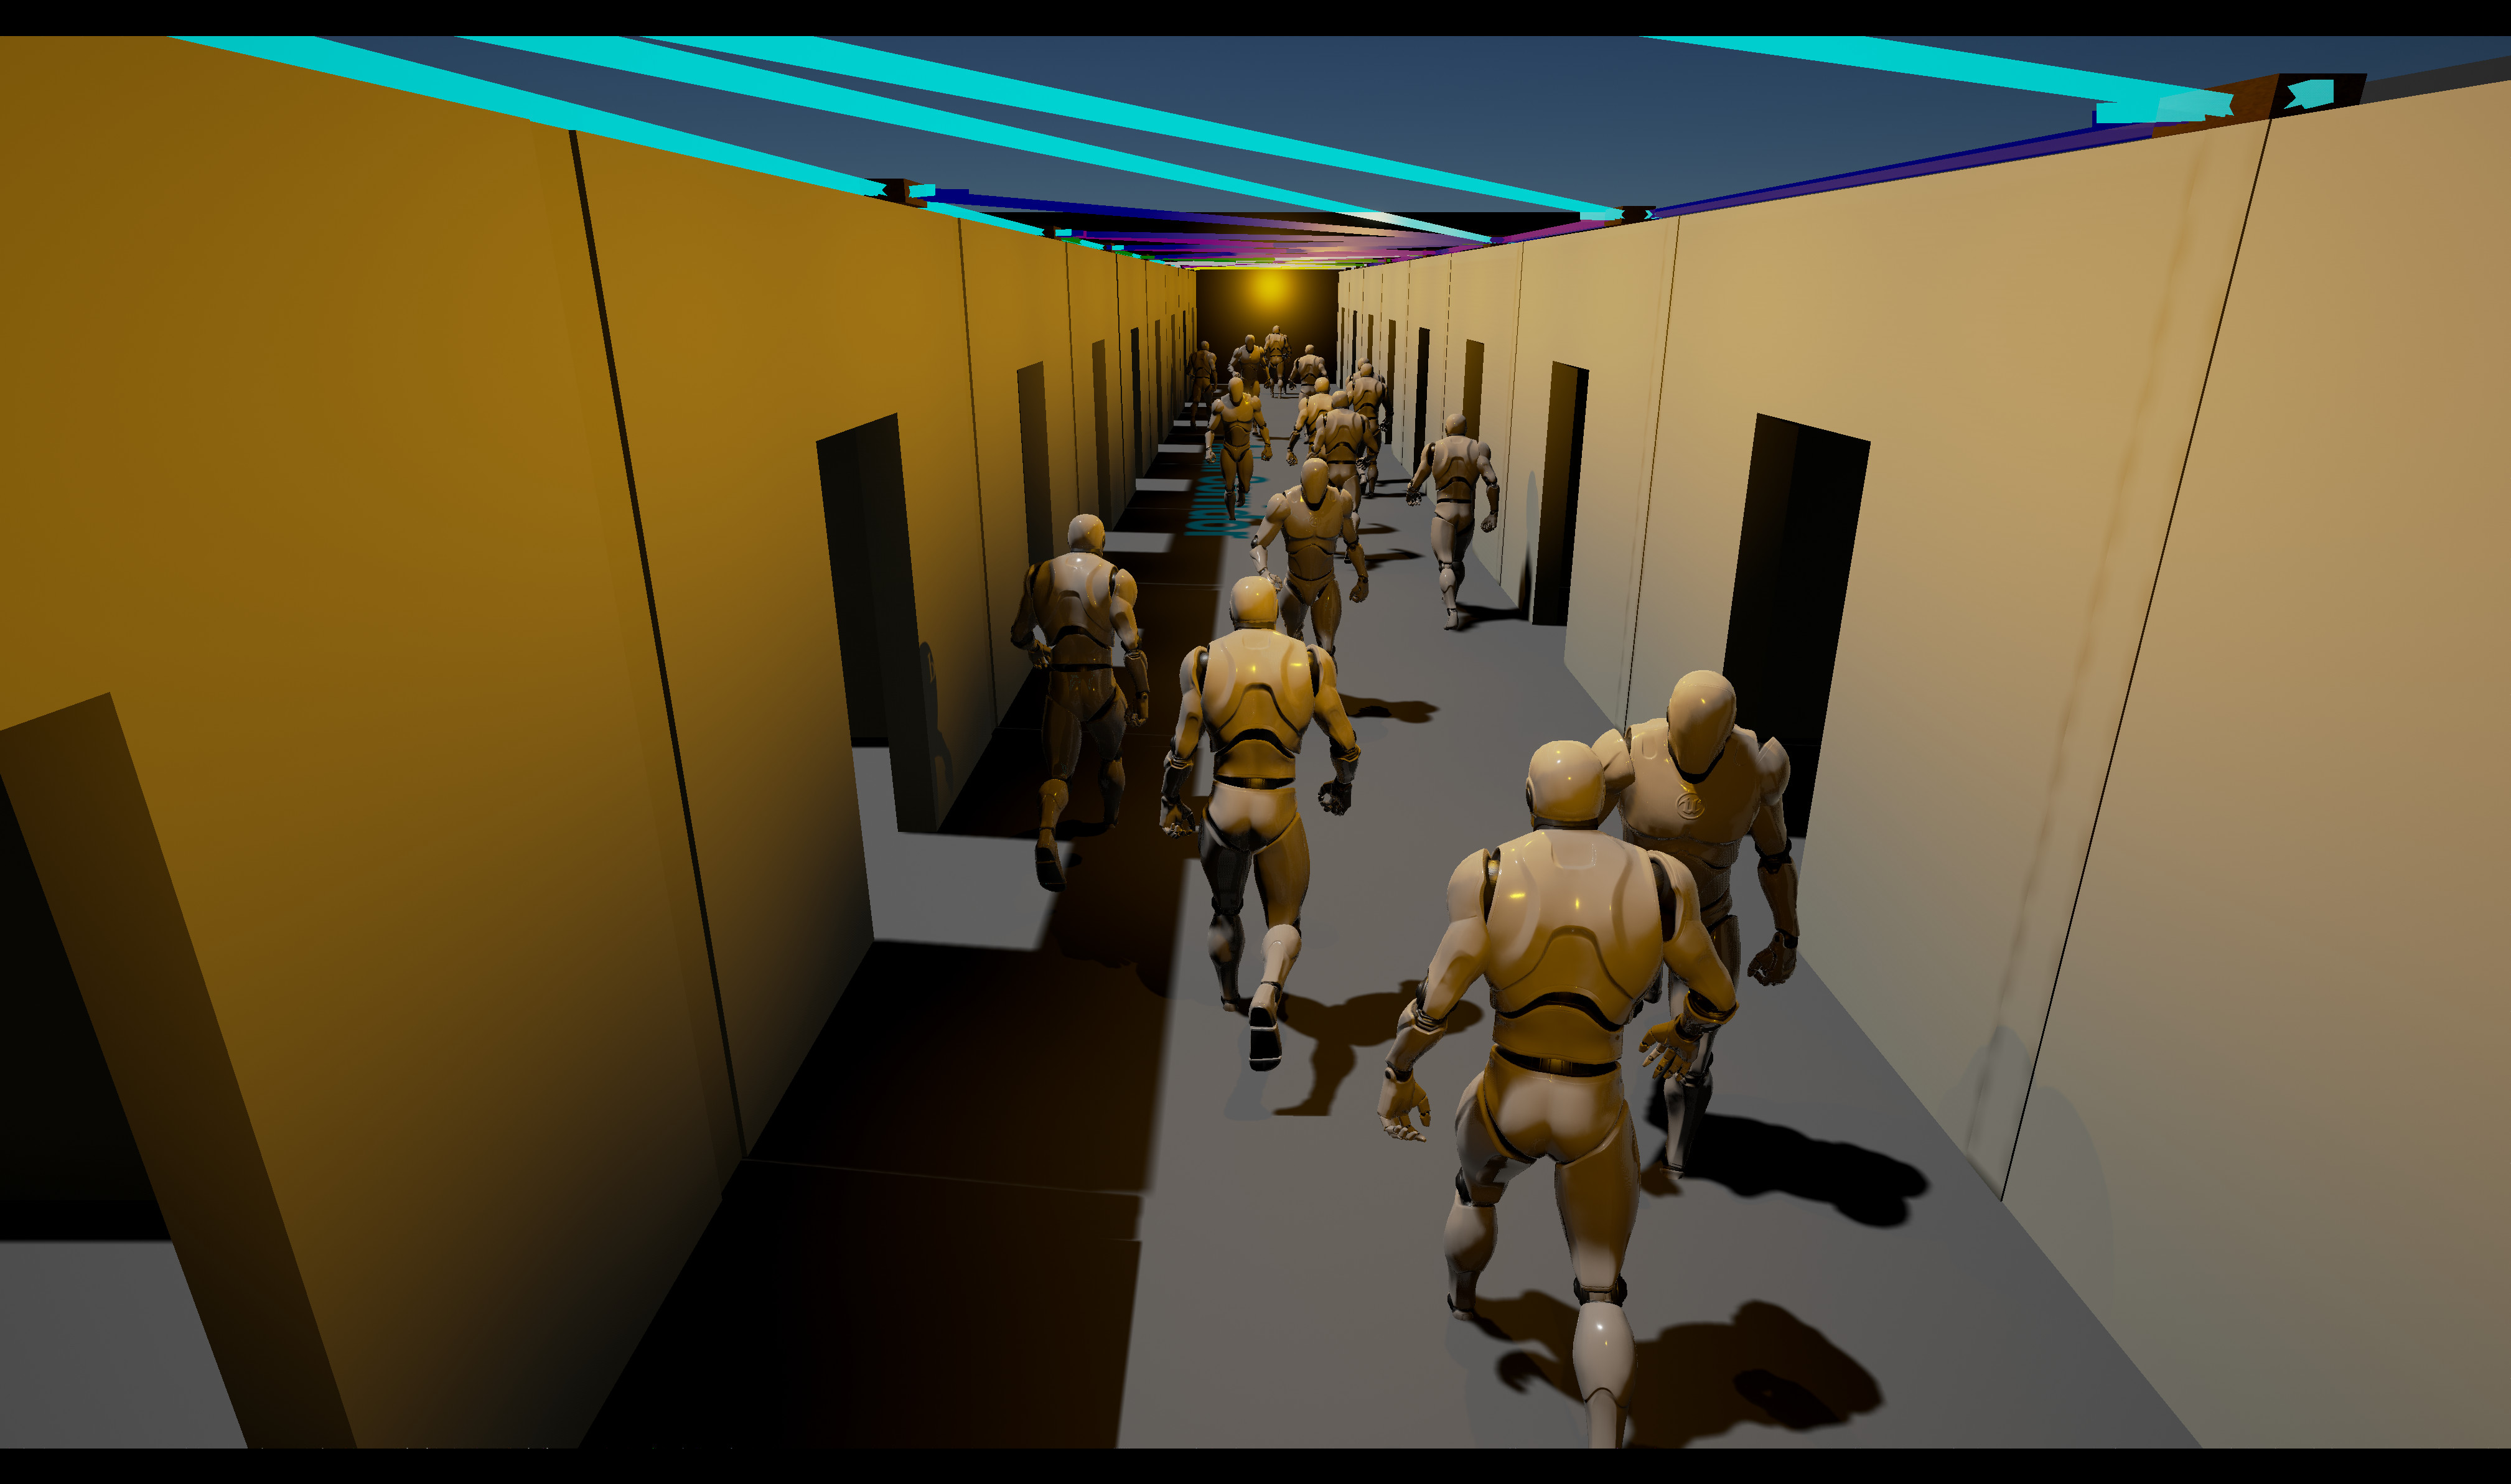
\includegraphics[height=2.6cm]{imgs/Camera.jpg}
    \label{fig:camera1_view}
  }
  \caption{15 people walking up and down the virtual corridor, triggering motion sensors}
  \label{fig:views}
\end{figure*}


\subsection{Corridor Design}
\label{sub:Constructing the corridor}
We created a virtual corridor based on a real corridor within our building, measuring 20x 1.5 meters, with 5 doors spaced evenly on either side. Along the corridor we placed 15 nodes with lights and conical motion sensors attached to the ceiling facing the floor directly below, shown in figure \ref{fig:corridor_layout}.

To construct the corridor, we used pre-existing models for walls, doorways and lights, making it quick to build or modify. In addition to these, we've created several new models for nodes and a variety of sensors, which can be composed together to create different sensing devices. A drag-and-drop interface is used to place nodes within the newly built 3D environment. The node model is based on a small box with 3 coloured lights, representing the typical LED outputs available on devices, such as the TelosB mote.

The next step was to create the nodes in the Cooja simulator, compiling and loading node application code. Using the IDs Cooja assigns to these nodes, the virtual representations were assigned matching IDs. This is especially important when certain applications are loaded on particular nodes, or when node IDs are used programmatically e.g., for location, routing or ordering.

\subsection{Lighting Algorithm}
\label{sub:Lighting Algorithm}
For demonstrative purposes, we developed a basic lighting algorithm based on our needs described previously. The algorithm, shown as pseudo code in figure \ref{fig:algorithm}, and developed further in figure \ref{fig:algorithm2}, waits for a motion detection event before illuminating its light for 5 seconds and notifying its closest neighbours. If it receives a message from a neighbour, it checks that it's adjacent, before illuminating its light for 3 seconds. The second variation attempts to build upon this algorithm, improving the lighting efficiency, using the simulator to test and experiment.

Using this as a base, we expect to test and iterate the algorithm based on our findings from our ``What if?'' scenarios.
\begin{figure}
\begin{verbatim}
  wait (event):
    if event == network:
      if msg.src + 1 == me or msg.src - 1 == me:
        turn_on_light(3000)
    if event == PIR:
      turn_on_light(5000)
      alert_neighbours()
\end{verbatim}
\caption{Lighting algorithm psuedo-code}
\label{fig:algorithm}
\end{figure}
\begin{figure}
\begin{verbatim}
  wait (event):
    if event == NETWORK and msg.dst == me:
      turn_on_light(5000)
      if msg.src + 1 == me:
        dir = FORWARD
      else if msg.src - 1 == me:
        dir = BACKWARD

    if event == PIR:
      turn_on_light(5000)
      if dir == FORWARD:
        alert_neighbour(FORWARD)
      else dir == BACKWARD:
        alert_neighbour(BACKWARD)
\end{verbatim}
\caption{Lighting algorithm psuedo-code with direction}
\label{fig:algorithm2}
\end{figure}



\subsection{``What if?'' scenarios}
\label{sub:Creating test scenarios}
When testing CPS deployments, ``what if'' questions about how the system will perform will naturally arise, such as ``what if we move or increase/decrease the number of nodes?'', or ``what if there are multiple people?'', or ``what if we place sensors differently or use more/less sensitive ones?''. Being able to quickly test and understand what happens to a system in these different scenarios is key to improving its reliability and efficiency.

In order to test our lighting application we devised several test scenarios to test both basic and complex situations for which we expect the system to perform correctly with; the complexity of a scenario increases as the number of agents in the scene increases and the pattern of movement changes from simple start to end directions, thus becoming more difficult to visualise and debug conceptually.

Using Ard\'{a}n, we are able to directly control a person in the virtual space, directing them down the corridor and observing, from multiple angles, the lighting algorithm reacting to their presence. This provides ultimate control in creating dynamic and new test scenarios, allowing developers to run around without any of the drawbacks of performing the same tests in real-life, such as fatigue, health and safety and time.

We also have the ability to adjust the number and placement of nodes within the environment, enabling us to test different configurations and determine which works best and fits our requirements.

Unlike the real world, using Ard\'{a}n we are able to pause the entire simulation, giving developers more time to understand the state of the network and virtual world at a particular point in time, before stepping through or continuing the simulation. On top of this, we are also able to change our view point between the cameras placed in the virtual world or move freely about within it to fully capture and understand the state of the environment whilst the simulation and world are paused, otherwise not possible in recorded videos of a real-world deployment.

Tests:
\begin{enumerate}
  \item One person
    \begin{itemize}
      \item Walks from end to end
      \item Walks from room to room
      \item Walks, stops, walks opposite direction
    \end{itemize}
  \item Multiple people
  \begin{itemize}
    \item Two agents walk from opposite ends
    \item Multiple agents walk in different patterns
  \end{itemize}
  \item Number and Placement of nodes
  \begin{itemize}
    \item 6 nodes, evenly spaced
    \item 6 nodes, with additional sensors placed facing doors
    \item 12 nodes, evenly spaced
  \end{itemize}
\end{enumerate}



\section{Evaluation}
To prove useful for a developer our system needs to scale to support large networks whilst ensuring synchronised behaviour at real-time or faster. To demonstrate the scalability of Ard\'{a}n, we designed a case study based on managing automated lighting in a typical office corridor, illustrated in figure \ref{fig:views}. Within the corridor we placed the sensor nodes and motions sensors. As people walk through a motion sensor, the relevant device is triggered and turns on its light before notifying its neighbours. When neighbours receive a notification they too turn on, providing a path of light illuminating around the walker. This task provides a non-trivial challenge for designing and testing applications that can deal with various scenarios that could occur, including multiple people walking in different directions, entering/exiting for different areas and people stopping/loitering.

The tests were run on the following spec machine: Xeon E5 1650 6Core with HT, 16GB RAM, 256GB SSD and a sufficiently powerful (MSI GeForce GTX 970) graphics card to support the game engine, otherwise, slow response times between the simulator and 3D game engine would cause the simulation to stall and drop below real-time performance.

\subsection{Co-simulator Performance} % (fold)
\label{sub:co_simulator_performance}

% subsection co_simulator_performance (end)
The results in figure \ref{fig:simulator_scalability} show that Ard\'{a}n can support up to 200 sensor nodes running at real-time with the simulator staying reliably synchronised with the game engine. Beyond this, the simulator performance degrades quickly and synchronisation is lost.

\begin{figure}[ht]
  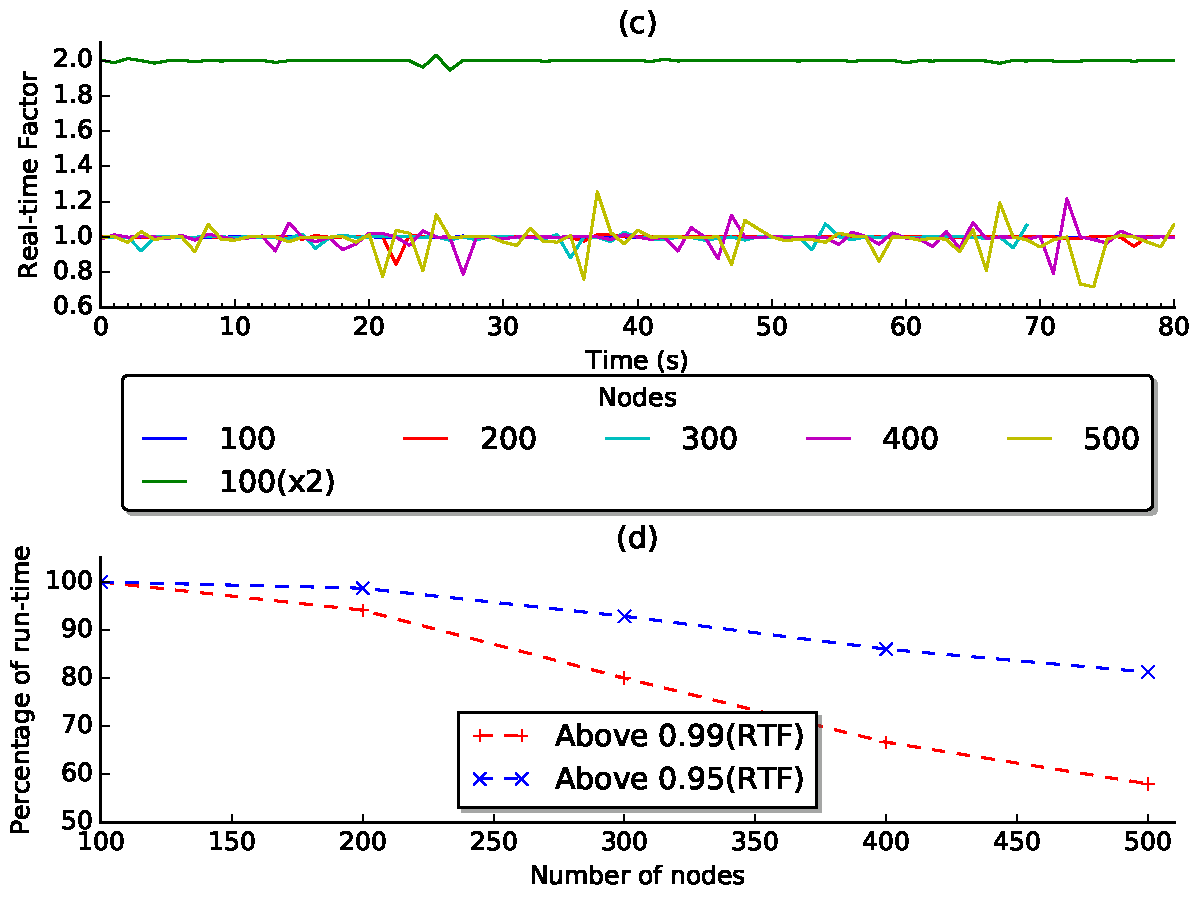
\includegraphics[width=0.5\textwidth]{plots/plot2.pdf}
  \caption{Figure (a) shows how the simulator speed fluctuates over time. Figure (b) shows the percentage of the total run time which the simulation maintains above 99\% and 95\% of its target speed.}
  \label{fig:simulator_scalability}
\end{figure}

Extending further, we also performed tests on running Ard\'{a}n at faster than real-time, at 200\% speed. In this mode, the game engine and its physics engine match the speed of the simulator, resulting in all activity increasing in speed, as opposed to simply increasing the walking speed of individuals. The results in figure \ref{fig:simulator_scalability} show that roughly half the number of nodes can be simulated in time with the game engine, with little fluctuation.

\subsection{Faster-than-real-time Performance} % (fold)
\label{sub:faster_than_real_time_performance}

% subsection faster_than_real_time_performance (end)

% \section{Requirements}
% \label{sec:Requirements}
% Define the list of key requirements described in workshop paper.

% \section{Framework} % (fold)
% \label{sec:framework}

% \subsection{CPS Simulation} % (fold)
% \label{sub:cps_simulation}

% \subsection{Virtual World Simulation} % (fold)
% \label{sub:virtual_world_simulation}
% % subsection virtual_world_simulation (end)
% % subsection cps_simulation (end)

% \subsection{Communication Model} % (fold)
% \label{sub:communication_model}
% % subsection communication_model (end)

% \subsection{Time} % (fold)
% \label{sub:time}
% % subsection time (end)
% % section framework (end)

% \section{Co-simulation} % (fold)
% \label{sec:co_simulation}

% \subsection{Performance} % (fold)
% \label{sub:performance}

% \subsection{Discussion} % (fold)
% \label{sub:discussion}

% subsection discussion (end)
% subsection performance (end)
% section co_simulation (end)

% \section{Features}
% Ard\'{a}n\footnote{Ard\'{a}n, pronounced ``awrd-awn'', is the Gaelic word for platform.} combines a high-performance 3D game engine, Unreal Engine 4, with an existing multi-level sensor network simulator, Cooja, to provide an end to end solution for testing real sensor network applications in virtual world environments. The rest of this section describes the novel key features and high-level design of Ard\'{a}n.

% Ard\'{a}n provides developers with a rich tool-set to control and observe the simulation environment, including 3D design and placement, time-control, phenomena-on-demand and visualisation.

% \subsection{3D design and placement}
% \label{sub:3D design and placement}
% A key part of many sensor network projects is understanding how many and where to place devices within the environment to achieve some desired objective, such as coverage, reliability or detection accuracy. Using Ard\'{a}n developers are able to easily scale up or down the size of the network and move devices around the environment to test different configurations.

% \subsection{Time Control}
% \label{sub:Time Control}
% Unlike in real world deployments, developers have the power to control time in the simulated world. Developers can: stop-the-clock, freezing both the simulation and world in time, whilst giving them full control over what they see, allowing more time to observe the environment and move between points of interest; slow down time, giving developers more time to observe or control the simulation; or even speed up time, providing desired results in considerably less time.

% \subsection{Phenomena-on-demand}
% \label{sub:Phenomena-on-demand}
% In order to fully test sensor network applications in the real-world, developers often need to wait for or even force desired phenomena to occur and then observe how their system reacts. However, exercising control over the real-world can be a difficult and time-consuming challenge, and sometimes not possible (e.g., fire), due to health and safety concerns.

% Using Ard\'{a}n, developers can take direct control of a virtual person or script intelligent virtual crowds to carry out tasks, such as walking between points, avoidance, following or interacting with objects. Figure \ref{fig:views} shows people walking up and down a corridor, avoiding each other's path. Unlike using trace data, genuine or created, developers can easily tweak scenarios, such as moving sensors, people or adjusting behaviour, to test subtle or significant variations. Developers can also create scenarios that are difficult or dangerous to reproduce in the real world, such as emergency situations, and repeatedly test their applications without risk.

% \subsection{Visualisation}
% \label{sub:Visualisation}
% Ard\'{a}n provides developers tools to overlay visualisations of network and sensor meta-information on top of the virtual world to help understand how the network is running, allowing developers to see information such as how network paths form as packets are sent, as well as transmissions, receptions, interruptions. In figure \ref{fig:views}, sending devices are highlighted with a circle and receiving devices are connected by an arrow to the sender, each device is represented with its own colour, to help differentiate simultaneous transmissions.

% \subsection{Virtual Sensors and Actuators}
% \label{sub:Virtual Sensors and Actuators}
% Within Ard\'{a}n we have modeled several basic sensors and actuators, including motion detectors, buttons, lights and location. These act as virtual hardware for the simulated sensors, allowing the simulation to interact with the virtual world. Virtual sensors can be designed to model a real sensors behaviour, or be virtually improved, providing higher accuracy or more features, not possible with existing hardware.




\section{Summary} % (fold)
\label{sec:summary}

% section summary (end)


% \section{Design Goals}
% \label{sec:Design Goals / Requirements}

% \subsection{Exploit 3D game engine to simulate CPS environment}
% \label{sub:Virtual Environments}
% Exploiting the use of 3D game engines simulate CPS in a virtual environment.

% \subsection{Analysing CPS in a 3D virtual world}
% \label{sub:analysing_cps_in_a_3d_virtual_world}
% Developing new tools to view and analyse CPS in 3D virtual environments.

% \subsection{Analysing CPS in the real world using AR} % (fold)
% \label{sub:analysing_cps_in_the_real_world_using_ar}
% How can we use techniques developed from previous chapter and apply them to analysing real-world CPS using AR technology.

% subsection analysing_cps_in_the_real_world_using_ar (end)
% \subsection{Comparing and learning from Virtual vs Real-world executions}
% \label{sub:Trained environment Models}
% Exposing the run-time differences of different network runs, to discover insights, highlight issues or debug new code.
% Building more accurate and scenario specific environment models by cross-training using pre-deployment data, creating more accurate localised models on environmental data, such as people movement/interaction, device models, temperature, operation speed etc.

% \subsection{Formally specifiying rules and testing counterexamples}
% \label{sub:formal}